\documentclass[a4paper,12pt,italian]{article}
\usepackage[italian]{babel}
\usepackage[utf8]{inputenc}
\usepackage{graphicx}
\usepackage{caption}
\title{Progetto Basi di Dati: Database Ferramenta}
\author{Daniele Vergara, N46001562 \\ Facoltà di Ingegneria Informatica\\ Università "Federico II" di Napoli}
\date{}
\setcounter{tocdepth}{1}
\begin{document}
\maketitle

\tableofcontents
\section*{Introduzione e specifiche sui dati}

Si voglia progettare una base di dati per una piccola attività; nello specifico, in questo caso, trattasi di una ferramenta. La base di dati deve fare in modo da semplificare la vita quotidiana del proprietario e dei suoi dipendenti, sostituendo il vecchio sistema informativo e costruendo un solido sistema informatico a supporto del tutto. 
Essa deve ovviamente rispettare le proprietà ACID (Atomicità, Consistenza, Isolamento, Persistenza) e i dati stessi devono essere prontamente accessibili qualora ve ne sia il bisogno.\\ Le informazioni conservate devono essere quelle usuali di un esercizio quale la ferramenta, ovvero, il database deve memorizzare quelle relative ai: \\ \\

• \emph{Dipendenti}, che devono avere un determinato codice di riconoscimento, una mansione a cui sono assegnati, il progetto a cui partecipano (se affidato), un nome, un cognome ed una data di nascita.

• \emph{Materiali}, che si dividono in materiali posseduti e in materiali richiesti/in arrivo. Tutti i materiali devono possedere l'informazione sul tipo di materiale, la quantità ed il fornitore che attualmente lo procura. Sui materiali posseduti è bene sapere in che progetto sono attualmente utilizzati (se lo sono); dei materiali in arrivo, invece, si devono conservare i dati sulla data di arrivo e sulla data di spedizione.

• \emph{Macchinari}, sui quali si devono memorizzare le informazioni sul codice della macchina, sul tipo della macchina, del dipendente che abitualmente lo usa e del progetto in cui è impegnato (se lo è).

• \emph{Progetti}, i quali devono poter essere facilmente riconosciuti attraverso un codice identificativo, dei quali si conserva l'informazione sulla data di inizio, sulla data (prevista) di conclusione, sul nome (tipo) del progetto, sui materiali utilizzati, sulle macchine utilizzate (se il progetto necessita l'utilizzo di specifiche apparecchiature) e sui dipendenti che sono impegnati nello stesso.

• \emph{Clienti}, dei quali si devono memorizzare i dati sul nome, cognome e sul progetto che ha richiesto (se lo ha fatto).

• \emph{Fornitori}, che devono possedere un nome ed il materiale che attualmente forniscono.

• \emph{Vendite}, delle quali si vuole salvare l'oggetto venduto, a quale cliente, a che prezzo ed in quale data. \\ \\
Inoltre, esistono 4 categorie di utenti che devono interagire con la base di dati: il database administrator, l'amministrativo, il dipendente ed il cassiere. Per adesso li lasciamo così come sono, ne daremo in seguito una definizione precisa.

\section{La progettazione concettuale}
\subsection{Analisi delle entità e interconnessioni fra loro}
Per progettare una base di dati la prima cosa da fare è sicuramente quella di delineare quali sono le entità cardine che ne fanno parte (in questo caso le abbiamo dalle specifiche), valutare come sono interconnesse fra loro e stilare il cosiddetto diagramma entità/relazione, fornendo così quello che sarà il primo assaggio della base di dati che ne verrà fuori.
Nel nostro caso, prima di disegnare il diagramma E/R vero e proprio, abbiamo cercato di schematizzare i concetti principali in forma tabellare dando ad ognuno una descrizione più o meno approfondita e cercando di interpretare ogni concetto con quale altro fosse legato, in modo da intuire più o meno quali fossero le associazioni del rispettivo diagramma entità/relazione. \\
Ne è venuto fuori lo schema in Figura 1. \\
Dalla figura si evince naturalmente che, per esempio, il dipendente è collegato al progetto e che il materiale richiesto è collegato ad un fornitore. Senza dubbio, avremo un'associazione fra il dipendente e il progetto e tra il materiale richiesto e il fornitore, nello schema E/R. \\

\begin{center}
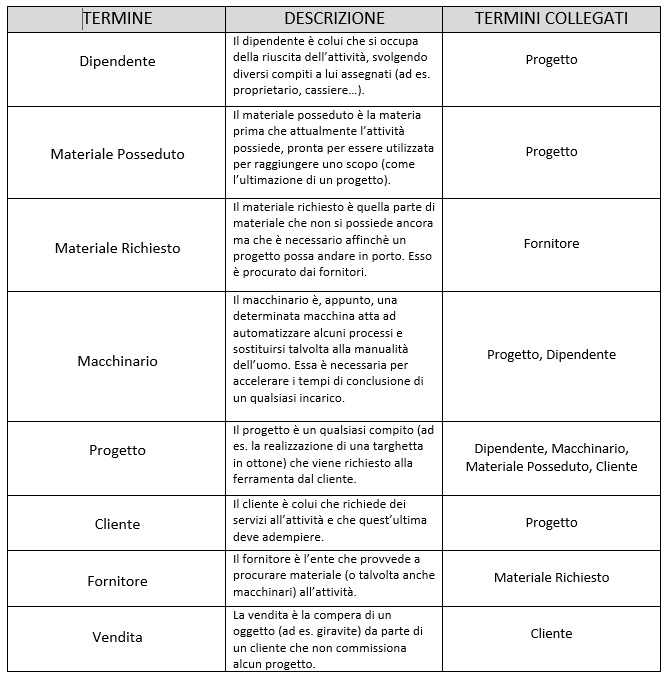
\includegraphics[width=15cm, height=17.1cm]{tabelladatabase.jpg}
\captionof{figure}{Tabella dei concetti\label{}}
\end{center}
 
\subsection{Il modello E/R Avanzato}
Il modello E/R Avanzato fornisce, come il termine suggerisce, una prima modellizzazione della nostra base di dati. E' "avanzato" poichè esso contiene le generalizzazioni e le specializzazioni (entità padre ed entità figlio) senza che esse siano state ancora risolte, operazione che compiremo successivamente, per tradurre il modello E/R avanzato in un modello E/R definitivo. \\
Il diagramma E/R avanzato è disegnato in Figura 2.

\begin{center}
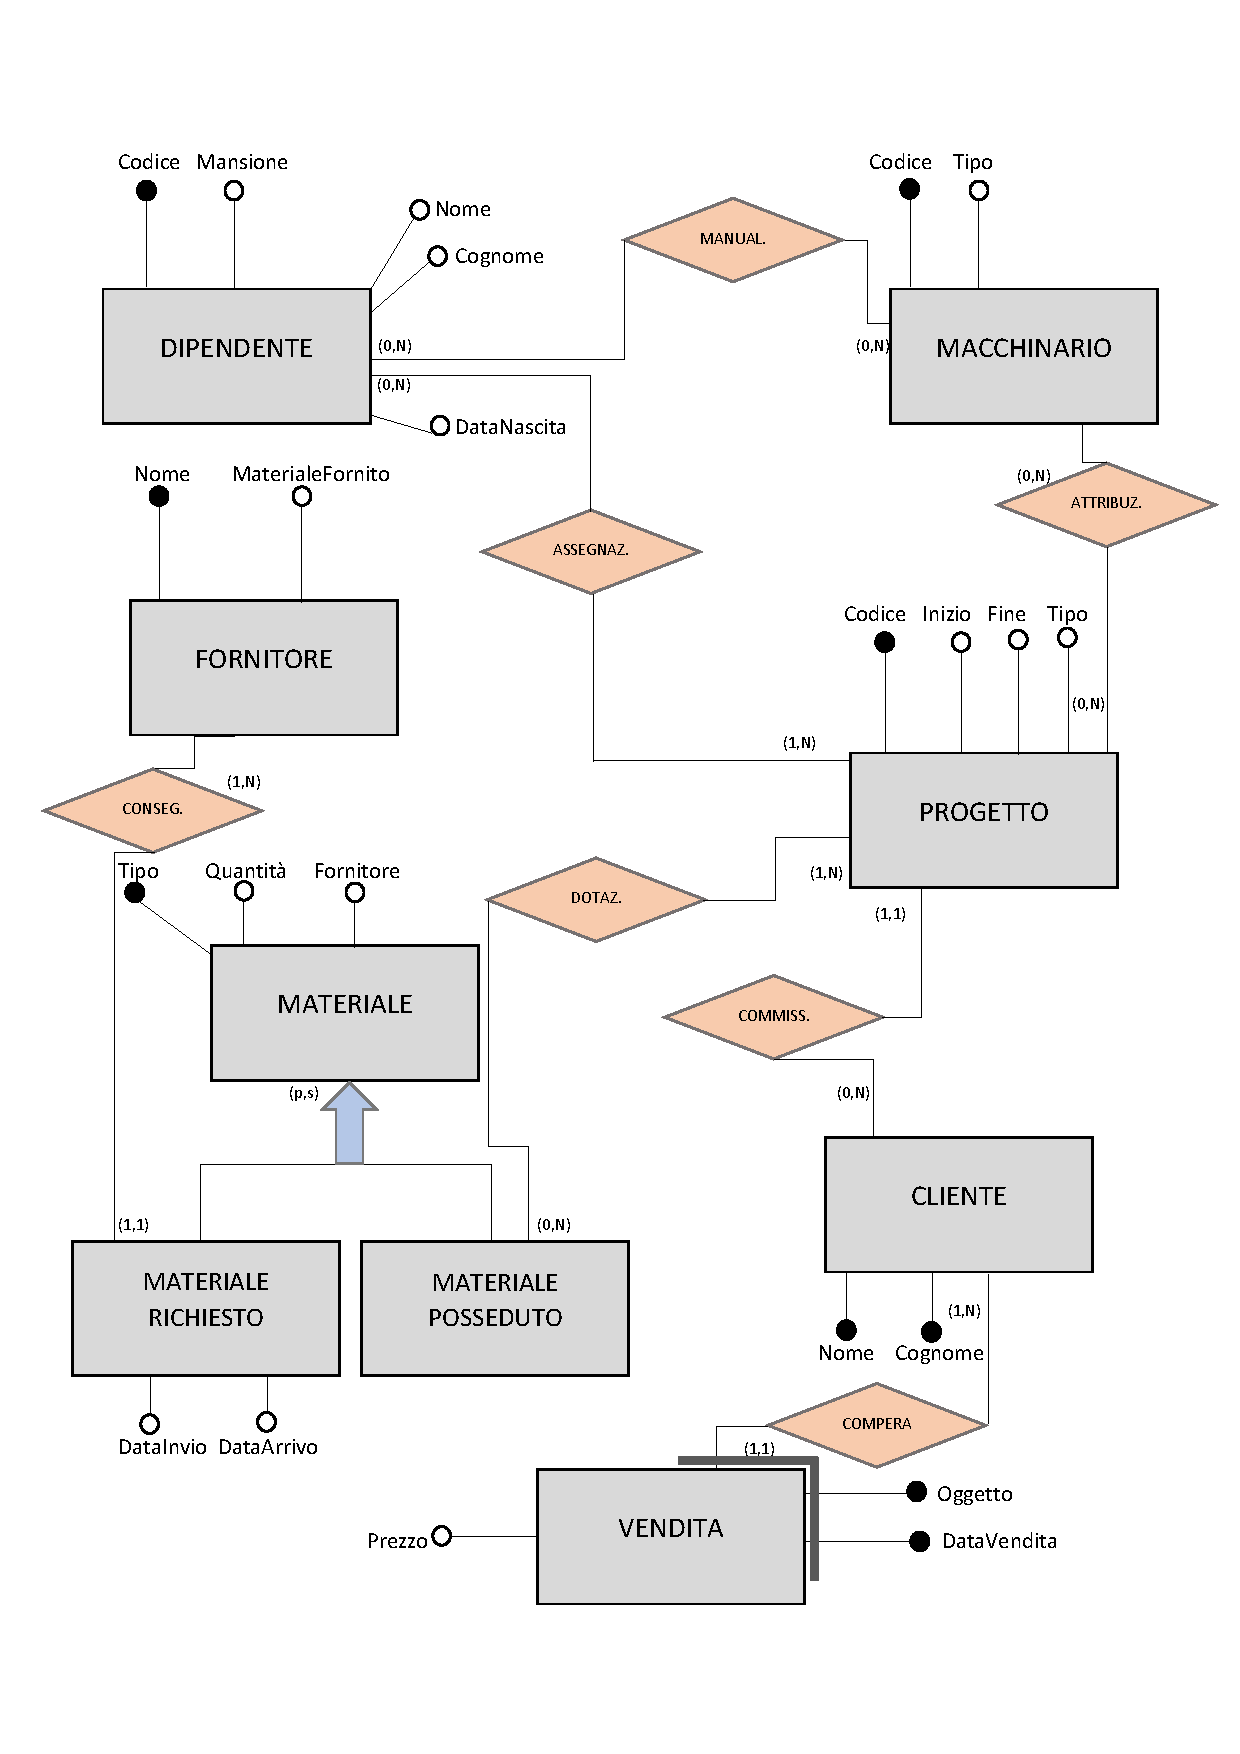
\includegraphics[width=15cm, height=18.6cm]{diagrammaeravanzato.pdf}
\captionof{figure}{Modello E/R Avanzato\label{}}
\end{center}
Notiamo dal modello che l'unica specializzazione presente è quella dei materiali, infatti i materiali si dividono - come da specifica - in materiali richiesti e posseduti. \\
In questo caso, l'entità Materiale è l'entità padre e le due entità figlie sono Materiale Posseduto e Materiale Richiesto. \\
E' una specializzazione parziale e sovrapposta: parziale perchè non tutti i materiali sono o in proprio possesso o in arrivo, ma potremmo avere anche dei materiali che non toccano minimamente una ferramenta (e che quindi essa non ha nè ordinato nè possiede. Cosa se ne farebbe una ferramenta del petrolio grezzo?). \\ 
E' sovrapposta perchè un materiale ordinato può benissimo essere un materiale che l'attività ha già e di cui vuole soltano incrementare la quantià (per esempio, se possediamo già dell'ottone ma ne necessitiamo di altro, lo ordianiamo ugualmente).

\subsection{Il modello E/R finale}
Risolvendo l'unica gerarchia del nostro modello entità/relazione avanzato, siamo in grado di ottenere quello definitivo e che useremo per passare alla progettazione logica della base di dati.
Il modello E/R finale è in Figura 3.

\begin{center}
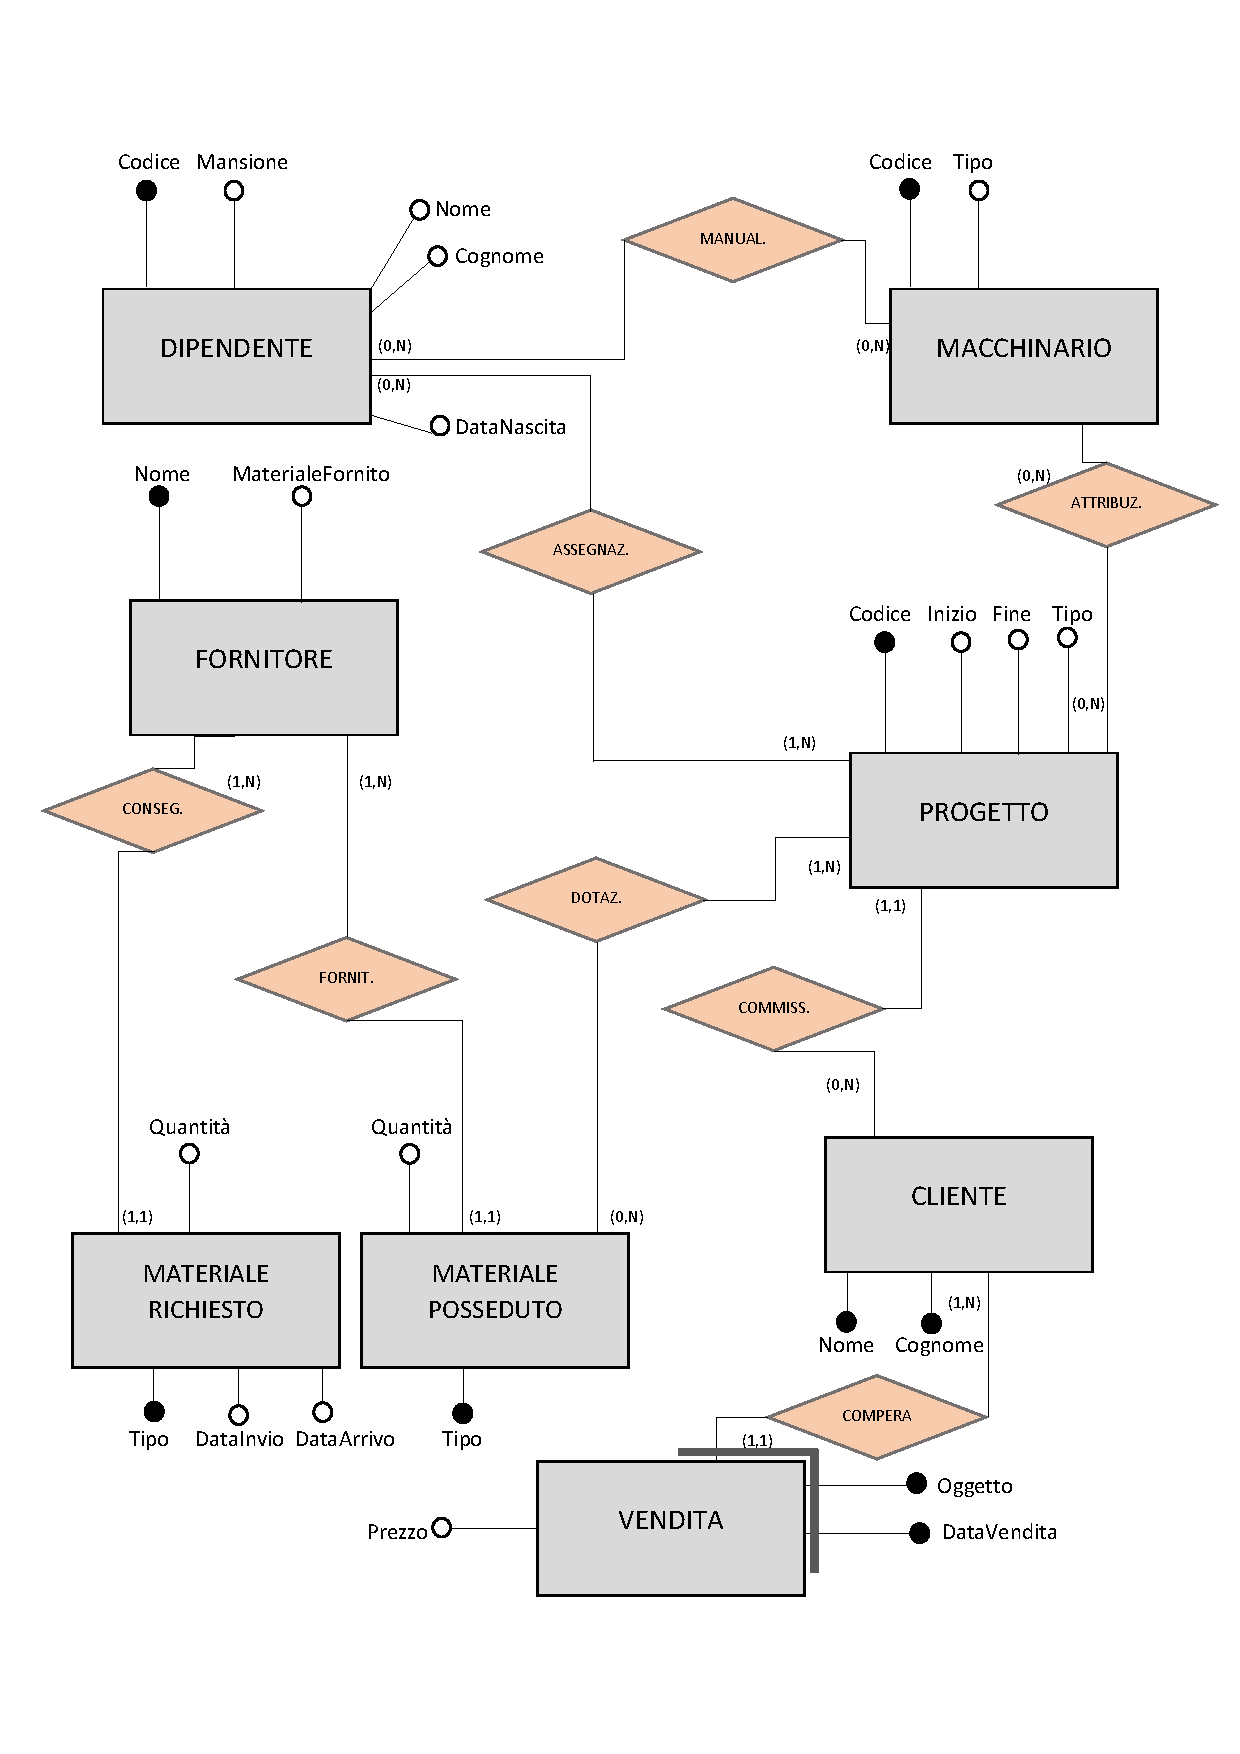
\includegraphics[width=15cm, height=18.6cm]{diagrammaerfinale.pdf}
\captionof{figure}{Modello E/R Finale\label{}}
\end{center}
Abbiamo deciso di risolvere la gerarchia accorpando l'entità padre in ognuna delle due entità figlie, poichè ci è sembrata la scelta più ragionevole da effettuare per semplicità e per efficienza.
Abbiamo inoltre aggiunto un'associazione in più rispetto al numero di associazioni presenti nel modello E/R avanzato, ovvero si è scelto di "connettere" anche l'entità Materiale Posseduto ai Fornitori, in modo da poter rendere l'attributo "Fornitori" dei materiali posseduti chiave esterna rispetto ai fornitori. \\ \\
Passiamo alle considerazioni sulla cardinalità attribuita alle varie associazioni tra le entità:  \\ \\
• Un dipendente può lavorare presso nessuno o più macchinari (0,N), mentre un macchinario può lavorare in automatico oppure essere associato a più dipendenti (0,N), ovvero la cardinalità dell'associazione MANUALITA' è di tipo molti a molti. \\
• Un dipendente può essere assegnato a nessuno o più progetti (0,N), mentre ad un progetto possono partecipare uno o più dipendenti (1,N), ovvero la cardinalità dell'assocazione ASSEGNAZIONE è di tipo uno a molti. \\
• Un fornitore può consegnare sotto richiesta da uno a più materiali (1,N), mentre il materiale quando richiesto può essere recapitato da uno ed un solo fornitore (1,1), ovvero la cardinalità dell'associazione CONSEGNA è tipo uno a molti. \\
• Un fornitore può allo stato attuale fornire uno o più materiali alla ferramenta (1,N), mentre il materiale attualmente in possesso può essere stato procurato da uno ed un solo fornitore (1,1), ovvero la cardinalità dell'assocazione FORNITURA è di tipo uno a molti. \\
• Un macchinario può essere neccessario per sviluppare nessuno o più progetti (0,N), mentre ad un progetto possono essere necessari nessuno o più macchinari per il suo compimento (0,N), ovvero la cardinalità dell'associazione ATTRIBUZIONE è di tipo molti a molti. \\
• Uno specifico materiale attualmente in possesso della ferramenta può essere utilizzato in nessuno o più progetti (0,N), mentre un progetto può far uso di uno o più materiali al fine di ottenere la sua ultimazione (1,N), ovvero la cardinalità dell'associazione DOTAZIONE è di tipo molti a molti. \\
• Un cliente può richiedere nessuno o più progetti all'attività (0,N), mentre un progetto può essere commissionato da uno ed un solo cliente della ferramenta (1,1), ovvero la cardinalità dell'associazione COMMISSIONE è di tipo uno a molti. \\
• Un cliente può effettuare da una a più compere nella ferramenta (1,N), mentre un acquisto può essere effettuato da uno ed un solo acquirente (1,1), ovvero la cardinalità dell'associazione COMPERA è di tipo uno a molti. \\ \\
Adesso che abbiamo chiare quali sono tutte le associazioni e quali cardinalità hanno, possiamo passare alla fase successiva: la progettazione logica.

\section{La progettazione logica}
La progettazione logica costituisce il punto che presenta la definizione dello schema relazionale della base di dati, con le appropriate relazioni e i vincoli adatti. \\
Essa si basa sulla trasformazione dello schema concettuale appena ricavato (il modello E/R finale) in un modello relazionale in modo da poter implementare fisicamente il database.

\subsection{La trasformazione dal modello concettuale a quello relazionale}
Utilizzando come riferimento lo schema entità/relazione finale di Figura 3 e prendendo in esame le precedenti considerazioni sulla cardinalità delle associazioni, siamo in grado di completare la trasformazione. \\
Ovviamente ogni entità diventa a sua volta una relazione, mentre invece per le associazioni utilizziamo le usuali regole di trasformazione delle associazioni, seguendo quelle che sono le loro cardinalità. \\
Gli identificatori delle entità, inoltre, diventano a loro volta chiavi delle relazioni che andremo a trovare (alcune le rinomineremo adeguatamente). \\
Trasformando il modello concettuale, otteniamo quello logico: \\ \\ \\
DIPENDENTI(\underline{Codice}, Mansione, Nome, Cognome, DataNascita) \\ \\
MACCHINARI(\underline{Codice}, Tipo) \\ \\
FORNITORI(\underline{Nome}, MaterialeFornito) \\ \\
MATERIALIRICHIESTI(\underline{Tipo}, Quantità, DataInvio, DataArrivo, NomeFornitore:FORNITORI) \\ \\
MATERIALIPOSSEDUTI(\underline{Tipo}, Quantità, NomeFornitore:FORNITORI) \\ \\
PROGETTI(\underline{Codice}, Tipo, Inizio, Fine) \\ \\
CLIENTI(\underline{Nome}, \underline{Cognome}, CodiceProgetto:PROGETTI) \\ \\
VENDITE(\underline{NomeCliente}:CLIENTI, \underline{CognomeCliente}:CLIENTI, \underline{Oggetto}, \underline{DataVendita}, Prezzo) \\ \\
MANUALITA(\underline{CodiceDipendente}:DIPENDENTI, \underline{CodiceMacchinario}:MACCHINARI) \\ \\
ASSEGNAZIONI(\underline{CodiceDipendente}:DIPENDENTI, \underline{CodiceProgetto}:PROGETTI) \\ \\
ATTRIBUZIONI(\underline{CodiceMacchinario}:MACCHINARI, \underline{CodiceProgetto}:PROGETTI) \\ \\
DOTAZIONI(\underline{TipoMateriale}:MATERIALIPOSSEDUTI, \underline{CodiceProgetto}:PROGETTI) \\ \\
Avendo a disposizione ora lo schema relazionale completo per la nostra base di dati, possiamo proseguire fino all'ultima fase: la progettazione fisica.

\section{La progettazione fisica}
La progettazione fisica è il terzo e ultimo step del processo che porterà a compimento la nostra base di dati. \\ In questa terza parte, come suggerisce il nome stesso, creeremo il vero e proprio database, definiremo le politiche di gestione vere e proprie e i vari vincoli di sicurezza, daremo la possibilià ad user specifici di operare sulla base di dati in una maniera che sarà protetta ed adatta al tipo di user che è attualmente connesso e realizzeremo un'istanza ovvero, procederemo al popolamento della base di dati. \\ \\
N.B. In questo progetto non tratteremo il dimensionamento della base di dati e daremo per scontato l'hardware e il sistema operativo del server che muoverà il tutto.

\subsection{Creazione dei ruoli}
Come già riportato su e nella prima parte del progetto, uno degli obiettivi che ci siamo posti è quello di rendere il database quanto più sicuro possibile e la prima via per raggiungere lo scopo è quello di creare dei ruoli. \\
Ciò è a beneficio dell'affidabilità perchè, per esempio, un cassiere della ferramenta che si connette al database per organizzare ciò che gli compete, deve poter modificare, appunto, solo la parte della base di dati che gli spetta, come quella relativa alle vendite. Non ha senso che un cassiere possa vedere e alterare le informazioni relative ai progetti o possa cambiare la mansione di un dipendente della ferramenta. Per questo, faremo in modo che i cassieri abbiano i privilegi per lavorare solo ed esclusivamente sulla relazione delle vendite, e così via. \\
Tiriamo fuori il linguaggio SQL e definiamo alcuni dei ruoli più importanti nella nostra attività. \\ \\
Incominciamo, ovviamente, col dichiarare il database administrator, il quale ha pieno controllo su ogni aspetto del database: \\ \\
\textbf{CREATE USER} FerramentaDBA \textbf{IDENTIFIED BY} admin; \\
\textbf{GRANT} dba \textbf{TO} FerramentaDBA; \\ \\
Una volta fatto ciò possiamo proseguire verso i ruoli più “limitati”. 
Andando in ordine decrescente di permessi, definiamo il ruolo “amministrativo”. Esso servirà per garantire alcune operazioni su specifiche tabelle ai dipendenti che ricoprono cariche amministrative all'interno della nostra attività. Essi devono poter visualizzare, inserire, modificare, cancellare tuple all'interno delle tabelle relative ai macchinari, ai materiali richiesti, ai materiali posseduti, ai fornitori, ai clienti. Devono inoltre poter gestire la forza lavoro, per cui è necessario che essi possano assegnare dipendenti ad un determinato progetto e/o ad uno specifica apparecchiatura, oltre che a congedarli e/o sostituirli (come di consueto, essi hanno il diritto di visualizzare quali dipendenti sono assegnati ad un macchinario o quali dipendenti stanno o sono in procinto di lavorare ad un progetto particolare). \\
A tale scopo quindi, esplicitiamo il ruolo: \\ \\
\textbf{CREATE ROLE} Amministrativo; \\
\textbf{GRANT CONNECT TO} Amministrativo; \\
\textbf{GRANT SELECT, INSERT, UPDATE, DELETE ON} FerramentaDBA.MACCHINARI \textbf{TO} Amministrativo; \\
\textbf{GRANT SELECT, INSERT, UPDATE, DELETE ON} FerramentaDBA.MATERIALIRICHIESTI \textbf{TO} Amministrativo; \\
\textbf{GRANT SELECT, INSERT, UPDATE, DELETE ON} FerramentaDBA.MATERIALIPOSSEDUTI \textbf{TO} Amministrativo; \\
\textbf{GRANT SELECT, INSERT, UPDATE, DELETE ON} FerramentaDBA.FORNITORI \textbf{TO} Amministrativo; \\
\textbf{RANT SELECT, INSERT, UPDATE, DELETE ON} FerramentaDBA.CLIENTI \textbf{TO} Amministrativo; \\
\textbf{GRANT SELECT, INSERT, UPDATE, DELETE ON} FerramentaDBA.MANUALITA \textbf{TO} Amministrativo; \\
\textbf{GRANT SELECT, INSERT, UPDATE, DELETE ON} FerramentaDBA.ASSEGNAZIONI \textbf{TO} Amministrativo; \\ \\
Passiamo adesso al secondo ruolo, quello del classico dipendente. Esso deve poter visualizzare, aggiungere, modificare o cancellare dei progetti. I dipendenti devono inoltre poter stabilire quali materiali e quali macchine sono più adeguate ad uno specifico progetto. \\
Dichiariamo quindi il ruolo Dipendente: \\ \\
\textbf{CREATE ROLE} Dipendente; \\
\textbf{GRANT CONNECT TO} Dipendente; \\
\textbf{GRANT SELECT, INSERT, UPDATE, DELETE ON} FerramentaDBA.PROGETTI \textbf{TO} Dipendente; \\
\textbf{GRANT SELECT, INSERT, UPDATE, DELETE ON} FerramentaDBA.ATTRIBUZIONI \textbf{TO} Dipendente; \\
\textbf{GRANT SELECT, INSERT, UPDATE, DELETE ON} FerramentaDBA.DOTAZIONI \textbf{TO} Dipendente; \\ \\
Infine, occorre definire il ruolo del cassiere. Il cassiere deve unicamente lavorare sulla tabella vendite come già specificato nell'esempio suddetto, in modo da poter gestire gli acquisti effettuati dai clienti dell'attività.\\ Quindi: \\ \\
\textbf{CREATE ROLE} Cassiere; \\
\textbf{GRANT CONNECT TO} Cassiere; \\
\textbf{GRANT SELECT, INSERT, UPDATE, DELETE ON} FerramentaDBA.VENDITE \textbf{TO} Cassiere; \\ \\
Procediamo verso la fase successiva.

\subsection{I create table} 
Di seguito abbiamo prodotto, in codice SQL, tutte le relazioni che abbiamo ricavato dalla trasformazione dal modello concettuale a quello logico. Senz'altro, ogni attributo avrà i suoi precisi vincoli e il suo specifico tipo (che abbiamo scelto in base al suo adattamento all'attributo stesso). \\
I comandi che producono le nostre tabelle sono i seguenti: \\ \\
\textbf{CREATE TABLE} DIPENDENTI( \\
Codice \textbf{CHAR(8)}, \\
Mansione \textbf{VARCHAR2(20)}, \\
Nome \textbf{VARCHAR2(25)}, \\
Cognome \textbf{VARCHAR2(25)}, \\
DataNascita \textbf{DATE}, \\
\textbf{PRIMARY KEY}(Codice) \\
); \\ \\
\textbf{CREATE TABLE} MACCHINARI( \\
Codice \textbf{CHAR(5)}, \\
Tipo \textbf{VARCHAR2(25)}, \\
\textbf{PRIMARY KEY}(Codice) \\
); \\ \\
\textbf{CREATE TABLE} FORNITORI( \\
Nome \textbf{VARCHAR2(25)}, \\
MaterialeFornito \textbf{VARCHAR2(25)}, \\
\textbf{PRIMARY KEY}(Nome) \\
); \\ \\
\textbf{CREATE TABLE} MATERIALIRICHIESTI( \\
Tipo \textbf{VARCHAR2(25)}, \\
Quantità \textbf{INTEGER}, \\
DataInvio \textbf{DATE}, \\
DataArrivo \textbf{DATE}, \\
NomeFornitore \textbf{VARCHAR2(25)}, \\
\textbf{PRIMARY KEY}(Tipo), \\
\textbf{FOREIGN KEY}(NomeFornitore) \textbf{REFERENCES} FORNITORI(Nome) \\
\textbf{ON DELETE} SET NULL \\
); \\ \\
\textbf{CREATE TABLE} MATERIALIPOSSEDUTI( \\
Tipo \textbf{VARCHAR2(25)}, \\
Quantità \textbf{INTEGER}, \\
NomeFornitore \textbf{VARCHAR2(25)}, \\
\textbf{PRIMARY KEY}(Tipo), \\
\textbf{FOREIGN KEY}(NomeFornitore) \textbf{REFERENCES} FORNITORI(Nome) \\
\textbf{ON DELETE} SET NULL \\
); \\ \\
\textbf{CREATE TABLE} PROGETTI( \\
Codice \textbf{CHAR(4)}, \\
Tipo \textbf{VARCHAR2(25)}, \\
Inizio \textbf{DATE}, \\
Fine \textbf{DATE}, \\
\textbf{PRIMARY KEY}(Codice) \\
); \\
\textbf{CREATE TABLE} CLIENTI( \\
Nome \textbf{VARCHAR2(25)}, \\
Cognome \textbf{VARCHAR2(25)}, \\
CodiceProgetto \textbf{CHAR(4)}, \\
\textbf{PRIMARY KEY}(Nome, Cognome), \\
\textbf{FOREIGN KEY}(CodiceProgetto) \textbf{REFERENCES} PROGETTI(Codice) \\
\textbf{ON DELETE} SET NULL \\
); \\ \\
\textbf{CREATE TABLE} VENDITE( \\ 
NomeCliente \textbf{VARCHAR2(25)}, \\
CognomeCliente \textbf{VARCHAR2(25)}, \\
Oggetto \textbf{VARCHAR2(30)}, \\
DataVendita \textbf{DATE}, \\
Prezzo \textbf{INTEGER}, \\
\textbf{PRIMARY KEY}(NomeCliente, CognomeCliente), \\
\textbf{FOREIGN KEY}(NomeCliente, CognomeCliente) \textbf{REFERENCES} CLIENTI(Nome, Cognome) \\ \textbf{ON DELETE} SET NULL \\
); \\ \\
\textbf{CREATE TABLE} MANUALITA( \\
CodiceDipendente \textbf{CHAR(8)}, \\
CodiceMacchinario \textbf{CHAR(5)}, \\
\textbf{PRIMARY KEY}(CodiceDipendente, CodiceMacchinario), \\
\textbf{FOREIGN KEY}(CodiceDipendente) \textbf{REFERENCES} DIPENDENTI(Codice) \\ \textbf{ON DELETE} SET NULL, \\
\textbf{FOREIGN KEY}(CodiceMacchinario) \textbf{REFERENCES} MACCHINARI(Codice) \\
\textbf{ON DELETE} SET NULL \\
); \\ \\
\textbf{CREATE TABLE} ASSEGNAZIONI( \\
CodiceDipendente \textbf{CHAR(8)}, \\
CodiceProgetto \textbf{CHAR(4)}, \\
\textbf{PRIMARY KEY}(CodiceDipendente, CodiceProgetto), \\
\textbf{FOREIGN KEY}(CodiceDipendente) \textbf{REFERENCES} DIPENDENTI(Codice) \\ \textbf{ON DELETE} SET NULL, \\
\textbf{FOREIGN KEY}(CodiceProgetto) \textbf{REFERENCES} PROGETTI(Codice) \\
\textbf{ON DELETE} SET NULL \\
); \\ \\
\textbf{CREATE TABLE} ATTRIBUZIONI( \\
CodiceMacchinario \textbf{CHAR(5)}, \\
CodiceProgetto \textbf{CHAR(4)}, \\
\textbf{PRIMARY KEY}(CodiceMacchinario, CodiceProgetto), \\
\textbf{FOREIGN KEY}(CodiceMacchinario) \textbf{REFERENCES} MACCHINARI(Codice) \\ \textbf{ON DELETE} SET NULL, \\
\textbf{FOREIGN KEY}(CodiceProgetto) \textbf{REFERENCES} PROGETTI(Codice) \\
\textbf{ON DELETE} SET NULL \\
); \\ \\
\textbf{CREATE TABLE} DOTAZIONI( \\
TipoMateriale \textbf{VARCHAR2(25)}, \\
CodiceProgetto \textbf{CHAR(4)}, \\
\textbf{PRIMARY KEY}(TipoMateriale, CodiceProgetto), \\
\textbf{FOREIGN KEY}(TipoMateriale) \textbf{REFERENCES} MATERIALIPOSSEDUTI(Tipo) \\ \textbf{ON DELETE} SET NULL, \\
\textbf{FOREIGN KEY}(CodiceProgetto) \textbf{REFERENCES} PROGETTI(Codice) \\
\textbf{ON DELETE} SET NULL \\
); \\ \\

\subsection{Popolamento della base di dati}

Una volta che abbiamo creato tutte le tabelle della base di dati, passiamo al loro popolamento. \\
Abbiamo di seguito il codice che inserisce le prime informazioni nelle tabelle che abbiamo generato: \\ \\
• Insert nella tabella DIPENDENTI \\
\textbf{INSERT INTO} DIPENDENTI \textbf{VALUES}('FD451236','Direttore','Dino','Vitale',\\to\_date('15-03-1950','dd-mm-yyyy')); \\
\textbf{INSERT INTO} DIPENDENTI \textbf{VALUES}('FD520101','Contabile','Francesco','Verdi',\\to\_date('28-10-1967','dd-mm-yyyy')); \\
\textbf{INSERT INTO} DIPENDENTI \textbf{VALUES}('AS478569','Tecnico','Antonio','Gianetta',\\to\_date('02-02-1970','dd-mm-yyyy')); \\
\textbf{INSERT INTO} DIPENDENTI \textbf{VALUES}('AS256901','Tecnico','Morgan','Virto',\\to\_date('10-08-1976','dd-mm-yyyy')); \\
\textbf{INSERT INTO} DIPENDENTI \textbf{VALUES}('CS102584','Cassiere','Angela','Tornisco',\\to\_date('04-05-1979','dd-mm-yyyy')); \\ \\
• Insert nella tabella MACCHINARI \\
\textbf{INSERT INTO} MACCHINARI \textbf{VALUES}('A4563','Cassa'); \\
\textbf{INSERT INTO} MACCHINARI \textbf{VALUES}('M2032','Pantografo'); \\
\textbf{INSERT INTO} MACCHINARI \textbf{VALUES}('M4587','Sist. tintometrico'); \\
\textbf{INSERT INTO} MACCHINARI \textbf{VALUES}('D0035','Duplicatrice'); \\ \\
• Insert nella tabella FORNITORI \\
\textbf{INSERT INTO} FORNITORI \textbf{VALUES}('Comitec','Ottone'); \\
\textbf{INSERT INTO} FORNITORI \textbf{VALUES}('Fision S.r.l.','Plexiglass'); \\
\textbf{INSERT INTO} FORNITORI \textbf{VALUES}('Tecniq','Alluminio'); \\
\textbf{INSERT INTO} FORNITORI \textbf{VALUES}('MOTV','Legno'); \\
\textbf{INSERT INTO} FORNITORI \textbf{VALUES}('Tizen S.r.l.','Plastica'); \\ \\
• Insert nella tabella MATERIALIPOSSEDUTI \\
\textbf{INSERT INTO} MATERIALIPOSSEDUTI \textbf{VALUES}('Alluminio',450,'Tecniq'); \\
\textbf{INSERT INTO} MATERIALIPOSSEDUTI \textbf{VALUES}('Legno',1100,'MOTV'); \\
\textbf{INSERT INTO} MATERIALIPOSSEDUTI \textbf{VALUES}('Ottone',1500,'Comitec'); \\
\textbf{INSERT INTO} MATERIALIPOSSEDUTI \textbf{VALUES}('Plexiglass',200,'Fision S.r.l.'); \\ \\
• Insert nella tabella MATERIALIRICHIESTI \\
\textbf{INSERT INTO} MATERIALIRICHIESTI \textbf{VALUES}('Ottone',700,to\_date('07-01-2013','dd-mm-yyyy'),\\to\_date('11-01-2013','dd-mm-yyyy'),'Comitec'); \\
\textbf{INSERT INTO} MATERIALIRICHIESTI \textbf{VALUES}('Plastica',300,to\_date('20-12-2012','dd-mm-yyyy'),\\to\_date('12-01-2013','dd-mm-yyyy'),'Tizen S.r.l.'); \\
\textbf{INSERT INTO} MATERIALIRICHIESTI \textbf{VALUES}('Alluminio',650,to\_date('05-01-2013','dd-mm-yyyy'),\\to\_date('13-01-2013','dd-mm-yyyy'),'Tecniq'); \\ \\
• Insert nella tabella PROGETTI \\
\textbf{INSERT INTO} PROGETTI \textbf{VALUES}('D4R7','Dupl. chiave',\\to\_date('05-01-2013','dd-mm-yyyy'),to\_date('06-01-2013','dd-mm-yyyy')); \\
\textbf{INSERT INTO} PROGETTI \textbf{VALUES}('AS83','Incisione',\\to\_date('07-01-2013,'dd-mm-yyyy')',to\_date('10-01-2013','dd-mm-yyyy')); \\
\textbf{INSERT INTO} PROGETTI \textbf{VALUES}('BC40','Tinteggiatura',\\to\_date('06-01-2013','dd-mm-yyyy'),to\_date('15-01-2013','dd-mm-yyyy')); \\ \\
• Insert nella tabella CLIENTI \\
\textbf{INSERT INTO} CLIENTI \textbf{VALUES}('Giuseppe','Arnoldi','AS83'); \\
\textbf{INSERT INTO} CLIENTI \textbf{VALUES}('Antonio','Russo','BC40'); \\
\textbf{INSERT INTO} CLIENTI \textbf{VALUES}('Chiara','Romanzi',NULL); \\
\textbf{INSERT INTO} CLIENTI \textbf{VALUES}('Emanuela','Di Giacomo','D4R7'); \\ \\
• Insert nella tabella VENDITE \\
\textbf{INSERT INTO} VENDITE \textbf{VALUES}('Chiara','Romanzi','Pila',\\to\_date('04-01-2013,'dd-mm-yyyy'),3); \\
• Insert nella tabella MANUALITA \\
\textbf{INSERT INTO} MANUALITA \textbf{VALUES}('AS478569','M2032'); \\
\textbf{INSERT INTO} MANUALITA \textbf{VALUES}('AS478569','D0035'); \\
\textbf{INSERT INTO} MANUALITA \textbf{VALUES}('CS102584','A4563'); \\
\textbf{INSERT INTO} MANUALITA \textbf{VALUES}('AS256901','M4587'); \\ \\
• Insert nella tabella ASSEGNAZIONI \\
\textbf{INSERT INTO} ASSEGNAZIONI \textbf{VALUES}('AS478569','AS83'); \\
\textbf{INSERT INTO} ASSEGNAZIONI \textbf{VALUES}('AS478569','D4R7'); \\
\textbf{INSERT INTO} ASSEGNAZIONI \textbf{VALUES}('AS256901','BC40'); \\
\textbf{INSERT INTO} ASSEGNAZIONI \textbf{VALUES}('FD520101','BC40'); \\ \\
• Insert nella tabella ATTRIBUZIONI \\
\textbf{INSERT INTO} ATTRIBUZIONI \textbf{VALUES}('M2032','AS83'); \\
\textbf{INSERT INTO} ATTRIBUZIONI \textbf{VALUES}('M4587','BC40'); \\
\textbf{INSERT INTO} ATTRIBUZIONI \textbf{VALUES}('D0035','D4R7'); \\ \\
• Insert nella tabella DOTAZIONI \\
\textbf{INSERT INTO} DOTAZIONI \textbf{VALUES}('Alluminio','D4R7'); \\
\textbf{INSERT INTO} DOTAZIONI \textbf{VALUES}('Ottone','AS83'); \\
\textbf{INSERT INTO} DOTAZIONI \textbf{VALUES}('Plexiglass','AS83'); \\ \\


\subsection{Le query sul database}
Abbiamo adesso alcuni dati memorizzati nel database della ferramenta: presentiamo qui una serie di interrogazioni alla base di dati al fine di testare la sua risposta di fronte alla necessità di recupero informazioni. \\ \\

\subsection*{Query n.1} 
Trovare il nome e il cognome di tutti i dipendenti della ferramenta: \\ \\
\textbf{SELECT} Nome, Cognome \\
\textbf{FROM} DIPENDENTI \\ \\

\subsection*{Query n.2} 
Trovare il tipo del macchinario il cui codice è “A4563”: \\ \\
\textbf{SELECT} Tipo \\
\textbf{FROM} MACCHINARI \\
\textbf{WHERE} Codice=”A4563” \\ \\

\subsection*{Query n.3} 
Trovare il tipo di tutti i progetti il cui codice inizia con la lettera D: \\ \\
\textbf{SELECT DISTINCT} Tipo \\
\textbf{FROM} Progetti \\
\textbf{WHERE} Codice LIKE ‘D\%’ \\

\subsection*{Query n.4}
Trovare i clienti dei quali la seconda lettera del nome è una ‘i’ e di cui il cognome termina per ‘e’. Ordinare poi il risultato in ordine decrescente per cognome (se si trovano due cognomi uguali, allora ordinare per nome): \\ \\
\textbf{SELECT DISTINCT} * \\
\textbf{FROM} CLIENTI \\
\textbf{WHERE} Nome=’\_i\%’ \textbf{AND} Cognome=’\%e’ \\
\textbf{ORDER BY} Cognome, Nome \textbf{DESC} \\ \\ 

\subsection*{Query n.5}
Trovare il codice dei progetti a cui sta attualmente partecipando il dipendente con codice “FD520101”: \\ \\
\textbf{SELECT} ASSEGNAZIONI.CodiceProgetto \\
\textbf{FROM} DIPENDENTI \textbf{JOIN} ASSEGNAZIONI \\ \textbf{ON} DIPENDENTI.Codice=ASSEGNAZIONI.CodiceDipendente \\
\textbf{WHERE} DIPENDENTI.Codice=’FD520101’ \\ \\

\subsection*{Query n.6}
Somma delle quantità di tutti i materiali in magazzino: \\ \\
\textbf{SELECT SUM}(Quantità) \textbf{AS} \\ SommaQuantità
\textbf{FROM} MATERIALIPOSSEDUTI \\ \\

\subsection*{Query n.7}
Trovare i macchinari che sono impegnati nel progetto “AS83” ma che non sono utilizzati nel progetto “BC40”: \\ \\
\textbf{SELECT} M.Codice, M.Tipo \\
\textbf{FROM} MACCHINARI M \textbf{JOIN} ATTRIBUZIONI A \textbf{ON} M.Codice=A.CodiceMacchinario \\
\textbf{WHERE} A.CodiceProgetto=’AS83’ \\ 
\textbf{EXCEPT} \\
\textbf{SELECT} M.Codice, M.Tipo \\
\textbf{FROM} MACCHINARI M \textbf{JOIN} ATTRIBUZIONI A \textbf{ON} M.Codice=A.CodiceMacchinario \\
\textbf{WHERE} A.CodiceProgetto=’BC40’ \\ \\

\subsection*{Query n.8}
Trovare qual è il prezzo medio di vendita dell’oggeto “Pila”: \\ \\
\textbf{SELECT AVG}(Prezzo) \textbf{AS} MediaPrezzo \\
\textbf{FROM} VENDITE \\
\textbf{WHERE} Oggetti=’Pila’ \\ \\

\subsection*{Query n.9}
Materiali in deposito di cui si possiede una quantità superiore alle 1500 unità (sapendo che si possiedono proprio 1500 unità del materiale Ottone): \\ \\
\textbf{SELECT} Tipo \\
\textbf{FROM} MATERIALIPOSSEDUTI \\
\textbf{WHERE} Quantità \begin{math} > \end{math} \textbf{ANY} ( \textbf{SELECT} Quantità \\
		                 \textbf{FROM MATERIALIPOSSEDUTI} \\	
			      \textbf{WHERE} Tipo=’Ottone’ ) \\ \\

\subsection*{Query n.10}
Per ogni progetto, trovare quanti dipendenti ne partecipano: \\ \\
\textbf{SELECT} P.Codice, P.Tipo \textbf{AS} Progetto, \textbf{COUNT}(A.CodiceDipendente) \textbf{AS} Dipendenti \\
\textbf{FROM} PROGETTO P \textbf{JOIN} ASSEGNAZIONI A \textbf{ON} P.Codice=A.CodiceDipendente \\	 
\textbf{GROUP} BY P.Tipo \\ \\

\subsection{I Trigger}
La creazione dei trigger è l'ultimo passo per l'ultimazione del progetto. I trigger sono fondamentali per automatizzare certi processi (essi matchano il paradigma "E-C-A") ed è bene quindi specificati. \\
La nostra base di dati prevede i seguenti trigger (DML):

\subsection*{Trigger n.1}
Il prezzo di un oggetto non può essere negativo. \\ \\
 {\fontsize{2mm}{3mm}1: create or replace trigger prezzononminore \\
 2: before insert on VENDITE \\
 3: for each row \\
 4: declare \\
 5: errore exception; \\
 6: begin \\
 7: if :new.Prezzo \begin{math} < \end{math} 0 \\
 8:	then raise errore; \\
 9: end if; \\
10: exception \\
11: when errore then raise\_application\_error(-20002,’Non puoi inserire un prezzo che sia negativo.’) \\
12: end; \\ \\}

\subsection*{Trigger n.2}
Prevediamo un meccanismo che mandi un messaggio di alert ogniqualvolta c'è scarsa disponibilità di un materiale (minore di 100).\\ \\
{\fontsize{2mm}{3mm} 1: create or replace trigger materialescarso \\
 2: after insert or update on MATERIALIPOSSEDUTI \\
 3: for each row \\
 4: declare \\
 5: messaggio exception; \\
 6: begin \\
 7: if :new.Quantità \begin{math} < \end{math} 100\\
 8: 	then raise messaggio; \\
 9: end if; \\
10: exception \\
11: when messaggio then raise\_application\_error(-20002,'Attenzione, c'è scarsità di materiale!') \\
12 end; 




\end{document}